\chapter{Grundlagen\label{chap2:Zweites-Kapitel}}

Um eine Konzeption und eine prototypische Umsetzung einer Search Engine in \gls{mcc} zu ermöglichen wird in folgendem Kapitel auf die architekturellen Hintergründe von \gls{mcc} eingegangen. Hierfür werden zu Beginn allgemein gültige Architektur-Prinzipien erläutert, welche auch bei der Integration einer Search Engine berücksichtigt werden müssen und somit bei der Auswahl eines geeigneten Konzeptes von Bedeutung sind.

Aufbauend auf den Architektur-Prinzipien wird die verwendete Microservice-Architektur erläutert, wobei neben einer allgemeinen Einführung in die Architektur auch auf die Kommunikation von Microservices untereinander eingegangen wird. Um mögliche Fehlkonzeptionen zu vermeiden, werden häufig auftretende Anti-Pattern aufgezeigt, welche unter Umständen zu monolithischen Seiteneffekten führen könnten.

Abschließend wird anhand von verschiedenen modernen Informationssystemen die Funktionalitäten der Volltextsuche gezeigt. Neben den unterschiedlichsten Anwendungsfällen für eine Volltextsuche werden auch die technischen Besonderheiten von Search Engines vorgestellt.

% Zum Verständnis und zur prototypischen Umsetzung der Integration einer Search Engine in \gls{mcc} werden die Grundlagen der Themen \glqq Microservice-Architektur\grqq{} und \glqq Search Engine\grqq{} benötigt. Diese werden in den folgenden Abschnitten behandelt. Zusätzlich zu den allgemeinen Grundlagen wird der Entwicklungsstand von \gls{mcc} vorgestellt, welcher für die Implementierung der Proof of Concept - Anwendung von Bedeutung ist.

\section{Software-Architekturen\label{sec2.1:Unterpunkt-1}}

\begin{quote}
    Die Software-Architektur eines Systems ist die Menge von Strukturen, die benötigt werden, um Entscheidungen über das System zu treffen, welche die Software-Elemente, die Relationen zwischen ihnen und die Eigenschaften von beiden betreffen. \textasciitilde{} Len Bass \cite{Bass.2013}
\end{quote}

Wie aus der Definition von Len Bass zu entnehmen ist, beschreibt eine Software-Architektur die Eigenschaften und Beziehungen von Software-Bausteinen zueinander \cite{Bass.2013}. Ein Software-Baustein wird hierbei als eine Teil-Komponente der gesamten Software betrachtet und wird bei der Erstellung einer Architektur als elementarer Bestandteil angesehen. Dabei wird ein Software-Baustein nicht näher spezifiziert, sondern als Komponente betrachtet, dessen konkrete Implementierung für die Architektur nicht von Bedeutung ist. Der Fokus einer Software-Architektur liegt auf den Schnittstellen der Software-Bausteine, über welche die Bausteine miteinander kommunizieren können.

\subsection{Architektur-Prinzipien\label{subsec2.1.1:Unterunterpunkt-1}}

Für das Erstellen einer guten Software-Architektur wurden von Vogel \cite{Vogel.2009} einige Grundprinzipien definiert. Diese Prinzipien sollten bei der Erstellung einer Software-Architektur beachtet werden.

\begin{description}
    \item[Lose Kopplung:]\hfill \\
    Inhalt

    \item[Hohe Kohäsion:]\hfill \\
    Inhalt

    \item[Entwurf für die Veränderung:]\hfill \\
    Inhalt

    \item[Separation of Concerns:]\hfill \\
    Inhalt

    \item[Information Hiding:]\hfill \\
    Inhalt

    \item[Abstraktion:]\hfill \\
    Inhalt

    \item[Modularität:]\hfill \\
    Inhalt

\end{description}

\subsection{Monolithische und verteilte Architekturen\label{subsec2.1.2:Unterunterpunkt-2}}

Inhalt

\begin{figure}[H]
    \centering
    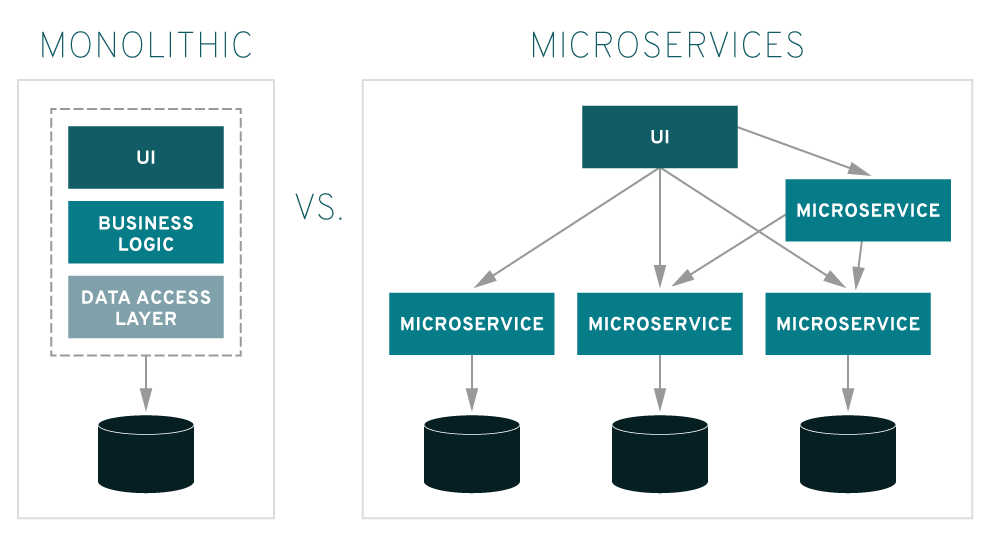
\includegraphics[width=0.7\linewidth]{images/monolithic-vs-microservices.png}
    \caption{3-Schichten-Architektur vs. Microservice-Architektur \cite{RedHatLimited.2021}}
    \label{fig:mono_vs_micro}
\end{figure}

\section{Microservice-Architektur\label{sec2.2:Unterpunkt-2}}

Für die Neugestaltung des \gls{mes} der Firma Enisco wird die Software auf einer verteilten Microservices-Architektur aufgebaut.

Die Kernelemente dieser Architektur sind die Microservices, welche der Modularisierung der Software dienen. Hierbei ist das unabhängige Deployment der Microservices eine wesentliche Eigenschaft. Die Möglichkeit Software modular aufzubauen, gibt es auch in monolithischen Architekturen. So helfen Ansätze, wie Klassen, Packages oder JARs in den Java-Umgebungen dafür eine Software in kleine Einheiten aufzuteilen und dadurch erweiterbar und wartbar zu machen. Das Problem ist jedoch, dass auch diese modularen Einheiten eine starke Abhängigkeit untereinander aufweisen und gemeinsam in einem Produktionsumfeld agieren müssen.

\subsection{Kommunikation zwischen Microservices\label{subsec2.2.1:Unterunterpunkt-1}}

Inhalt

\subsection{Vorteile\label{subsec2.2.2:Unterunterpunkt-2}}

Inhalt

\subsection{Microservice - Antipattern\label{subsec2.2.3:Unterunterpunkt-3}}

Inhalt

\section{Volltextsuche in modernen Informationssystemen\label{sec2.3:Unterpunkt-3}}

Inhalt

\subsection{Anwendungsfälle\label{subsec2.3.1:Unterunterpunkt-1}}

Inhalt

\subsection{Search Engines\label{subsec2.3.2:Unterunterpunkt-2}}

Inhalt